\documentclass[twocolumn, 10pt,a4j]{jsarticle}
\usepackage{amsmath}
\usepackage{here}
\usepackage[dvipdfmx]{graphicx}
\usepackage{url}
% プリアンブル
\title{\vspace{-2.5cm}制御系設計と実装}
\author{1610581 堀田 大地}
\date{2018/11/1}
\begin{document}
\maketitle{}
\section{課題}
% 課題
  \subsection{レポート課題~A}
  % 課題A
    \begin{enumerate}
      \item No.1 \\
        $T_{d}=$0.1-1.0のときの結果を図1,表1に示した.  
      \item No.2 \\
        $T_{d} \geq 0.8$以降で変化が見られるのは,式(1)の真数が
        0に近づくためだと考えられる.
      \item No.3 \\
        結果を図2,表2に示した.
    \end{enumerate}
    
    \begin{figure}[H]
      \centering
      % 図1
      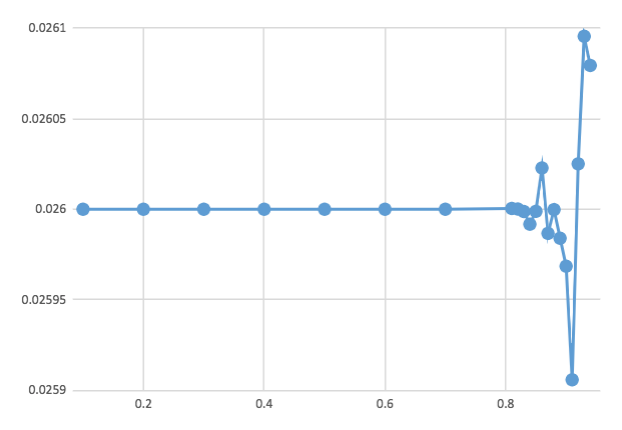
\includegraphics[width=7cm]{../img/A-no1.png}
      \caption{$T_{d}$を0.1から1.0まで変化させた結果.$T_{d} \geq 0.8$}から変化が見られる.
    \end{figure}

    \begin{figure}[H]
      \centering
      % 図1
      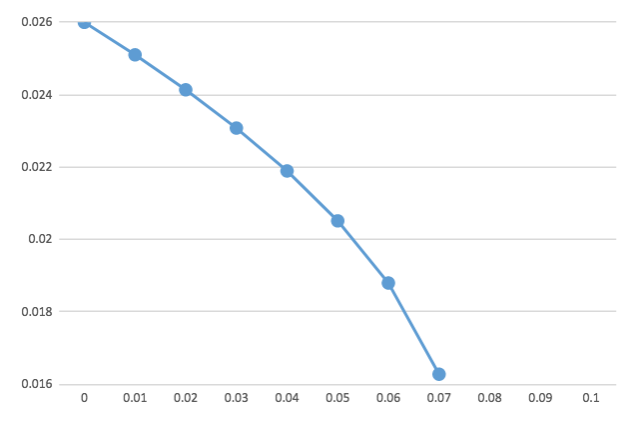
\includegraphics[width=7cm]{../img/A-no3.png}
      \caption{$T_{d}$を0.1から1.0まで変化させた結果.$T_{d} \geq 0.8$}から変化が見られる.
    \end{figure}

    \begin{table}
      \begin{center}
        \caption{$T_{d}$を0.1から1.0に変化させた時の(19)式の値}
        \begin{tabular}{|c|c|c|} \hline
          \footnotesize
            $T_{d}$ & $x(t_{d})$ & (19) \\ \hline
            0.1	& 3.5647 & 0.026 \\
            0.2	& 3.64092	& 0.026 \\
            0.3	& 3.64255	& 0.026 \\
            0.4	& 3.64258	& 0.026 \\
            0.5	& 3.64258	& 0.026 \\
            0.6	& 3.64258	& 0.02599 \\
            0.7	& 3.64258	& 0.02600 \\
            0.81 & 3.64258	& 0.02600 \\
            0.82 & 3.64258	& 0.02600 \\
            0.83 & 3.64258	& 0.02599 \\
            0.84 & 3.64258	& 0.02599 \\
            0.85 & 3.64258	& 0.02599 \\
            0.86 & 3.64258	& 0.02602 \\
            0.87 & 3.64258	& 0.02598 \\
            0.88 & 3.64258	& 0.02599 \\
            0.89 & 3.64258	& 0.02598 \\
            0.9 & 3.64258	& 0.02596 \\
            0.91 & 3.64258	& 0.02590 \\
            0.92 & 3.64258	& 0.02602 \\
            0.93 & 3.64258	& 0.02609 \\
            0.94 & 3.64258	& 0.02607 \\
            0.95 & 3.64258	& 0.02585 \\
            0.96 & 3.64258	& 0.02613 \\
            0.97 & 3.64258	& 0.02640 \\
            0.98 & 3.64258	& Null \\
            0.99 & 3.64258	& Null \\
            1 & 3.64258	& Null \\ \hline
        \end{tabular}
      \end{center}
    \end{table}

    \begin{table}
      \begin{center}
        \caption{$T_{d}$を0.1から1.0に変化させた時の(19)式の値}
        \begin{tabular}{|c|c|c|} \hline
          \footnotesize
          δ	& 正しい$x'(T_{d})$ & $\tau$ \\ \hline
          0 & 3.5647 & 0.0268 \\
          0.01 & 3.5547 & 0.0268 \\
          0.02 & 3.5447 & 0.0276 \\
          0.03 & 3.5347 & 0.0284 \\
          0.04 & 3.5247 & 0.0291 \\
          0.05 & 3.5147 & 0.0298 \\
          0.06 & 3.5047 & 0.0305 \\
          0.07 & 3.4947 & 0.0312 \\
          0.08 & 3.4847 & 0.0318 \\
          0.09 & 3.4747 & 0.0324 \\
          0.1 & 3.4647 & 0.0331 \\ \hline
        \end{tabular}
      \end{center}
    \end{table}

  \subsection{レポート課題~B}
  % 課題B
  P,PI制御における台車の応答,制御機の出力を図3,4に示した.
  外乱が無い場合の台車の応答は,P制御の方がPI制御に比較して短い時間で
  目標位置に到達している. また,PI制御は外乱がない場合もオーバーシュート量が
  大きくなった. 外乱がある場合,P制御は目標位置に到達できていないが,PI制御では
  外乱が無い場合と同じ時間で目標地点に到達できている. 
  \par よって,外乱が無い場合でオーバーシュートを小さくする必要があるときは
  P制御を用いるべきであり,現実世界で外乱が無い場合などほとんど無いので,そのような
  特例を除けばPI制御をも用いるのが妥当である.


  \begin{figure}[H]
    \centering
    % 図1
    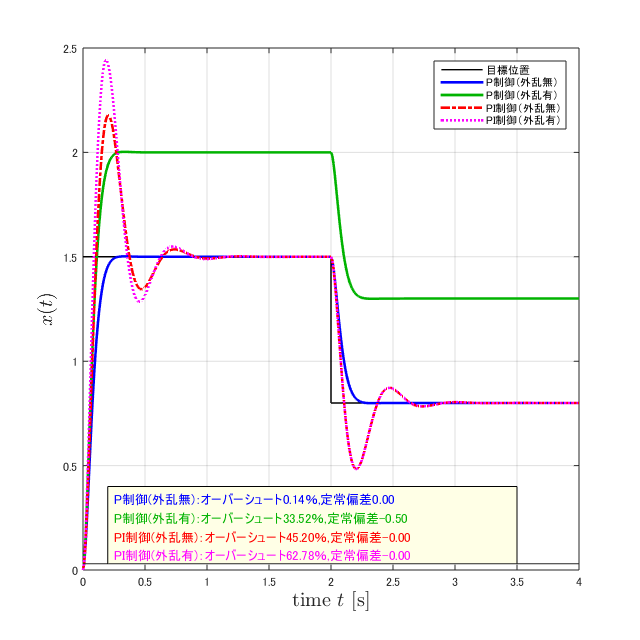
\includegraphics[width=7cm]{../img/B-1.png}
    \caption{$T_{d}$を0.1から1.0まで変化させた結果.$T_{d} \geq 0.8$}から変化が見られる.
  \end{figure}

  \begin{figure}[H]
    \centering
    % 図1
    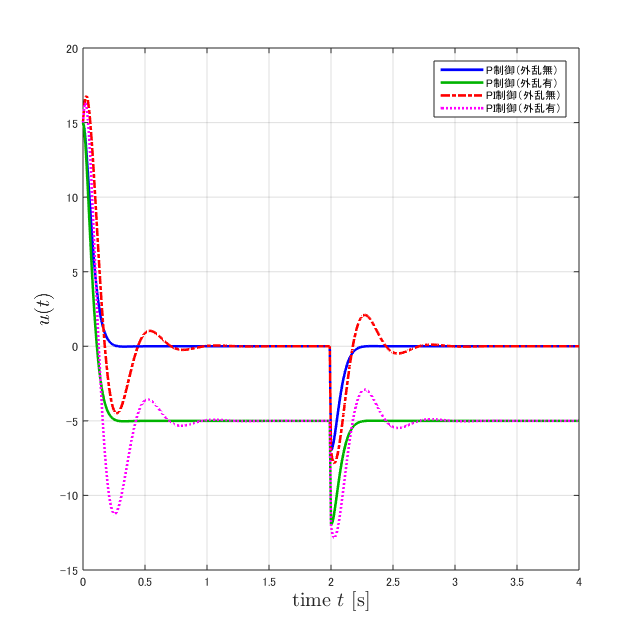
\includegraphics[width=7cm]{../img/B-2.png}
    \caption{$T_{d}$を0.1から1.0まで変化させた結果.$T_{d} \geq 0.8$}から変化が見られる.
  \end{figure}

  \subsection{レポート課題~C}
    % 課題C
    LQ制御の重み$q_{1}$の値に応じたシミュレーション,実機実験を比較した図を図5に示した.
    LQ制御の重み$Q$は,Q=(1, 1, 0.1, 1), (0.1, 1, 0.1, 1), (3, 1, 0.1, 1)と変化させた.
    $q_{1}$の値が大きくなるにつれて台車の位置が目標値に収束する時間が短くなっているが,
    同時に振り子の角度の振れ幅も大きくなっていた.
    \par また,評価関数は(3)であり,$q_{1}$と値が大きくなると,$x^{2}(t)$が小さくなり,
    積分値である面積が小さくなることがわかる. さらに,$q_{2}$の重みが小さくなり,$\theta^{2}(t)$
    の値が大きくなり,同様に積分値の面積であるのでオーバーシュートが大きくなり.
    よって,$q_{1}$の値が大きくなると,位置と目標値の間の面積が小さくなり台車の位置
    が目標値に早く収束し,振り子の角度と目標角度の間の面積が大きくなってオーバーシュートが大きくなる.

    \begin{eqnarray}
      \int_{0}^{\infty}(q_{1} x^{2}(t) + q_{2} \theta^{2(t)} + q_{3} \dot{x}^{2}(t) + q_{4}\dot{\theta}^{2}(t) + u^{2}(t) )dt
    \end{eqnarray}

  \subsection{レポート課題~D}
  % 課題D
    \begin{enumerate}
      \item 振り子の運動方程式. \\
        振り子の運動エネルギー,位置エネルギーは式(2),(3)であるので,
        ラグラジアン$L$は式(4)となる.式(5)のラグラジアンの運動方程式より,
        式(6)が得られる.
        \begin{eqnarray}
          T &=& \frac{1}{2} m l^{2} \dot{\theta}^{2} + \frac{1}{2} I \dot{\theta}^{2} \\
          V &=& mgl \cos \theta \\
          L &=& T - V  \\ \nonumber
          &=& \frac{1}{2} m l^{2} \dot{\theta}^{2} + \frac{1}{2} I \dot{\theta}^{2} - mgl \cos \theta \\
          \frac{d}{dt}\left( \frac{\partial L}{\partial \dot{\theta}} \right) - \frac{\partial L}{\partial \theta} &=& u \\
          (I + ml^{2})\dot{\dot{\theta}} - mgl \sin \theta &=& u
        \end{eqnarray}

      \item 線型表現. \\
        式(6)で角度$\theta$が小さいとき,$\$sin \theta = \theta$と近似すると,式(7)
        となる. この式を$\dot{\dot{\theta}}$について解くと式(8)となる.
        以上より,$\bf{x} = [\dot{\theta}, \theta]^{T}$とすると, 式(8)が得られる.
        よって,$A = \left[
          \begin{array}{cc}
            0 & \frac{mgl}{I+ml^{2}} \\
            1 & 0
          \end{array}
        \right]$,$B = \left[
          \begin{array}{c}
            \frac{1}{I+ml^{2}} \\
            0
          \end{array}
        \right]$となる.

        \begin{eqnarray}
          (I + ml^{2})\dot{\dot{\theta}} - mgl \theta = u \\
          \dot{\dot{\theta}} = \frac{mgl}{I + ml^{2}}\theta + \frac{1}{I + ml^{2}}u \\
          \frac{d}{dt}\dot{\bf{x}} = \left[
                                        \begin{array}{cc}
                                          0 & \frac{mgl}{I+ml^{2}} \\
                                          1 & 0
                                        \end{array}
                                      \right] \bf{x} + \left[
                                                        \begin{array}{c}
                                                          \frac{1}{I+ml^{2}} \\
                                                          0
                                                        \end{array}
                                                      \right]u
        \end{eqnarray}

    \end{enumerate}


\begin{thebibliography}{3}
\bibitem{}電気通信大学,知能機械高額基礎実験,実験テキスト,p14-25
\end{thebibliography}
\end{document}